\chapter{Evaluation}
This section describes {\dime} accuracy and comparison with other emulator.
All experiments were performed on an Intel Xeon CPU E5-2650 server with 16 hyper-threaded and CPUs operating at 2.60 GHz. Each application was executed from within a Linux/KVM virtual machine with 3 vCPUs and 6 GB RAM running Linux kernel 4.4.70 with huge page disabled.

\section{Verification of Correctness}
We evaluated {\dime} for correctness based on different scenarios and test cases.

\subsection{Page faults}
We have written a test program in C language, which takes number of pages as an argument and "malloc"ates the memory. Since we have disabled huge pages, default page size is 4kB. The program first accesses all the allocated pages in sequence and then access last 'x' pages. At the end of execution, test script extracts total number of page faults occurred from {\dime} procfs config file, \verb|/proc/dime_config|.

We setup {\dime} with following configurations: \verb|local_npages|=1000; \verb|latency_ns|=10000; \verb|bandwidth_bps|=10000000000000000 (infinite). We allocate 2000 pages in test program that runs under emulator. Table \ref{tab:last_page_access_test} shows test results where we vary number of last pages accessed ('x') and calculate the page faults. As expected, the number of page faults are constant till x=900, i.e. ~2000 for first iteration of page access, and starts increasing after x=1100 by ~100. It shows that 900 last pages were already in local memory and no page fault raised for those. Since FIFO page replacement policy is used, the page fault count jumps by ~1000 at x=1100, because all local pages are evicted from list once again. The extra ~100 page faults that we see in all test cases are of test program text section which are always required in local memory for program execution.

\begin{table}[]
	\centering
	\caption{Last 'x' pages access test results}
	\label{tab:last_page_access_test}
	\begin{tabular}{cccc}
		\hline
		\textbf{\begin{tabular}[c]{@{}c@{}}Number of last\\ pages accessed\end{tabular}} & \textbf{\begin{tabular}[c]{@{}c@{}}Total execution\\ time (us)\end{tabular}} & \textbf{\begin{tabular}[c]{@{}c@{}}Number of\\ page faults\end{tabular}} & \textbf{\begin{tabular}[c]{@{}c@{}}Average time taken\\ per page fault (us)\end{tabular}} \\ \hline
		0 & 50,989.50 & 2,099.00 & 24.29 \\
		100 & 51,113.50 & 2,102.50 & 24.31 \\
		200 & 51,145.00 & 2,100.50 & 24.35 \\
		300 & 50,733.50 & 2,099.50 & 24.16 \\
		400 & 50,289.00 & 2,100.50 & 23.94 \\
		500 & 49,209.50 & 2,099.50 & 23.44 \\
		600 & 47,617.50 & 2,100.50 & 22.67 \\
		700 & 48,605.00 & 2,102.00 & 23.12 \\
		800 & 49,755.50 & 2,102.00 & 23.67 \\
		900 & 46,625.00 & 2,101.00 & 22.19 \\
		1000 & 53,386.00 & 2,339.50 & 22.82 \\
		1100 & 72,608.00 & 3,182.00 & 22.82 \\
		1200 & 73,316.50 & 3,269.00 & 22.43 \\
		1300 & 77,493.50 & 3,388.00 & 22.87 \\
		1400 & 79,642.50 & 3,491.50 & 22.81 \\
		1500 & 77,371.50 & 3,595.50 & 21.52 \\
		1600 & 82,422.00 & 3,695.50 & 22.30 \\
		1700 & 81,398.50 & 3,801.50 & 21.41 \\
		1800 & 86,171.50 & 3,910.00 & 22.04 \\
		1900 & 84,671.50 & 3,999.50 & 21.17 \\
		2000 & 90,360.50 & 4,107.00 & 22.00 \\ \hline
	\end{tabular}
\end{table}

\subsection{Cache flush requirement} \label{ssec:cache_flush_eval}
As explained in Section \ref{ssec:tlb_flush}, it is mandatory to flush TLB after every page table update. To verify this, we built a C program which allocates 1000 pages, i.e. 1000x4KB memory, and accesses only two bytes from two different pages alternatively 1000 times per byte. We modified {\dime} to protect only the allocated 1000 pages, i.e. only data section of the process and not the text section. We set \verb|local_npages|=1 so that last page always get protected for each page fault. It was found that if we do not flush TLB after protecting previously accessed page, the page fault count was around $\sim$200, which is much less than expected count of 2000. After we patched the module with TLB flush, the page fault count was exactly 2000 as expected.


\subsection{Delay injection accuracy} \label{ssec:delay_eval}
As described in section \ref{sec:delay_injection}, there are multiple ways to inject a delay \cite{timers}. We evaluate each method by injecting delays from 0 to 10000 nanoseconds. In Linux kernel, different clock sources \cite{clock_sources} can be used to measure time \cite{measure_timelapse}. We use Time-stamp counter (TSC~\cite{tsc}) source available in x86 architecture (TSC library \cite{tsclibrary}) to measure actual injection time in each case. We sampled the measurement over 100 times and calculated the average for each method. Figure \ref{fig:lat_accuracy} show the plot between delay injected (x-axis) and actual measured delay (y-axis). The \verb|usleep_range| function deviates most from idle delay injection since it involves interrupts and is nondeterministic delay between the given range. \verb|usleep_range| is not useful for small amount of delays, since the error is higher for delays less than 2000ns. The \verb|ndelay| function injects delay with much higher accuracy for lower values of delay, but the error increases linearly for higher values of delay. Our custom busy loop method of delay injection works most accurately with almost constant error of 70ns for any value of delay.

\begin{figure}[t]
	\centering
	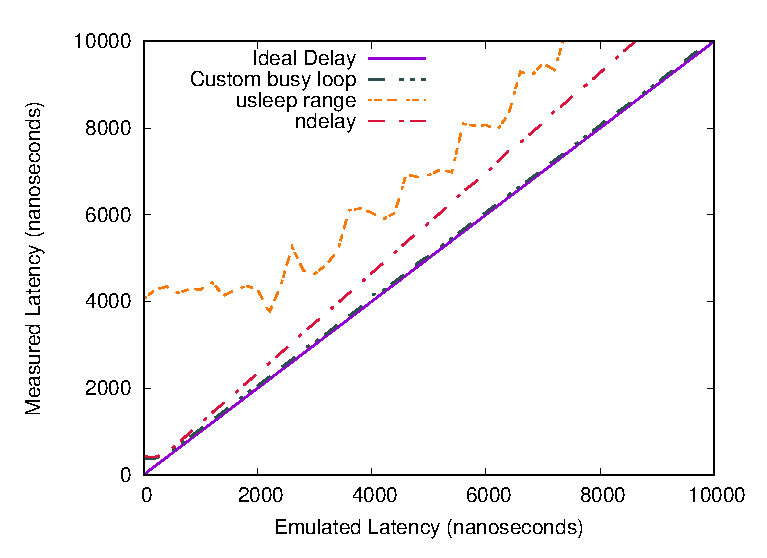
\includegraphics{evaluation/lat_accuracy.eps}
	\caption{Accuracy of delay injection methods.}
	\label{fig:lat_accuracy}
\end{figure}

\subsection{Average time per page fault}
From Table \ref{tab:last_page_access_test}, average time taken per page fault is 22.87${\mu}s$. The expected time was 20${\mu}s$ (two times one-way latency, 2x1000 ns), the error is of 2.87${\mu}s$. Since the time is measured from user space, the error contains context switching and interrupt handling time.


\section{Application Throughput Test}
The application performance degrades which are running under emulator. To verify if performance degradation is valid based on emulator configuration, we vary each parameter by keeping other constant. We ran Redis~\citep{redis} server under emulator with 3 server threads. We used YCSB\cite{ycsb} benchmarking to generate the load. Redis client with 10 client threads, running on another VM, generates 1Gb of workload with equal amount of read and write operations. In Figure \ref{fig:vary_config_localmem}, we vary amount of local memory available for Redis server in percent of workload by keeping network bandwidth and latency constant. Results show that server throughput increases as available local memory increases.

Figure \ref{fig:vary_config_latency} shows the test results where bandwidth and local memory is constant while latency is changed. As we can see, the server throughput increases as latency decreases.

Similar results were observed when Memcached~\cite{memcached} was used in place of Redis.

\begin{figure}[t]
	\centering
	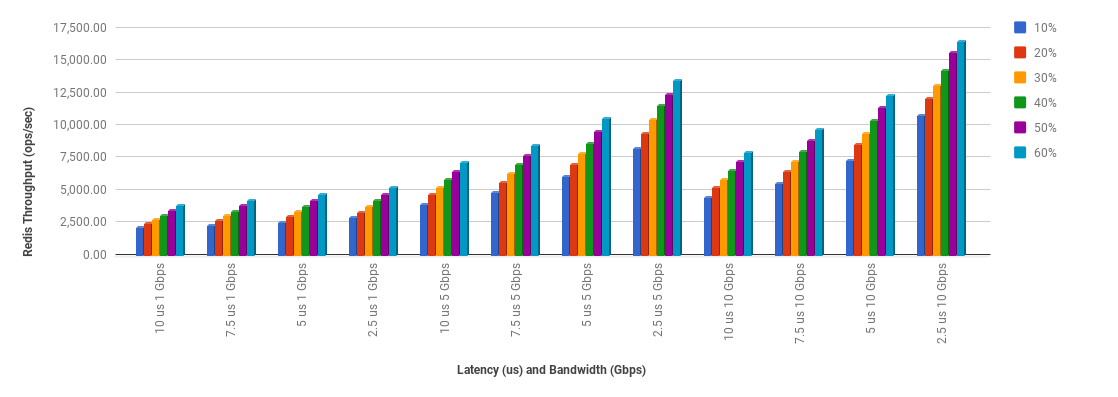
\includegraphics[width=\linewidth]{evaluation/vary_config_throughput_local_mem.png}
	\caption{Redis throughput with constant latency and bandwidth, varying local memory}
	\label{fig:vary_config_localmem}
\end{figure}

\begin{figure}[t]
	\centering
	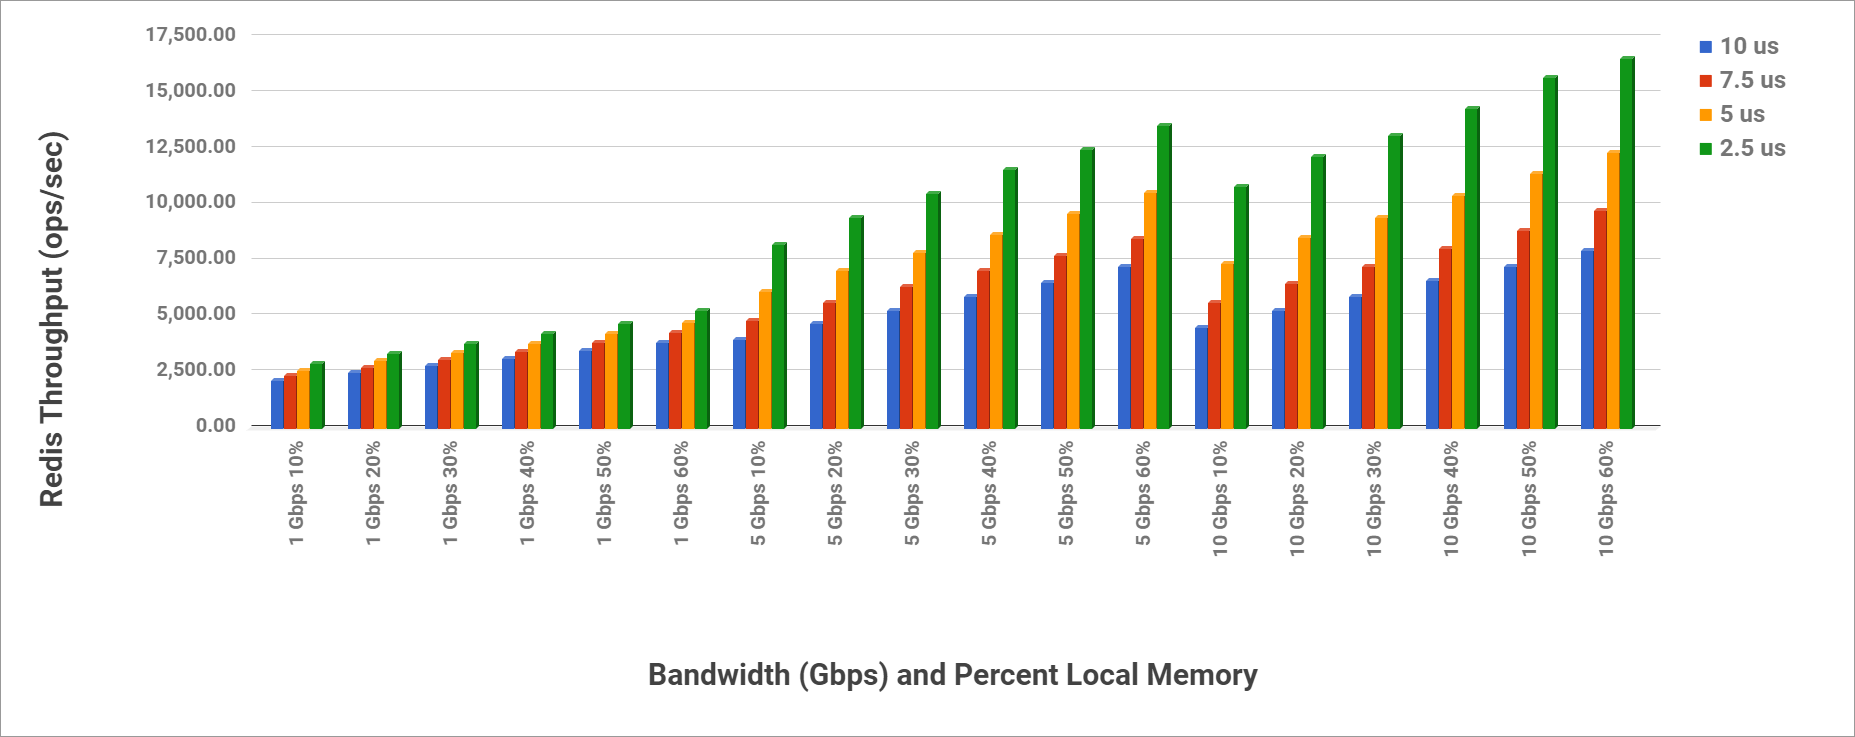
\includegraphics[width=\linewidth]{evaluation/vary_config_throughput_latency.png}
	\caption{Redis throughput with constant bandwidth and percent local memory, varying latency}
	\label{fig:vary_config_latency}
\end{figure}

\section{Comparison with System-wide Emulator}
The existing emulators (e.g. the one developed in \cite{Gao}) emulates memory at system granularity. The entire system memory is partitioned into remote and local memory and user has no control over which portion of memory should reside on remote or local. In contrast, {\dime} emulates remote memory at the granularity of a process. {\dime} also has page level control over amount of local/remote memory and can specify custom page replacement policy. The allocated local memory is fixed and other applications running on the system outside the emulator has no effect on emulation. On the other hand, system-wide emulator cannot eliminate the effect of other applications running simultaneously outside the emulator. There are also other factors which affects the emulation accuracy in case of system-wide emulator, e.g. page cache usage, local memory consumed by other processes running in background, swap-out threshold, etc.

We compare the performance degradation of popular real world applications (Redis~\cite{redis} and Memcached~\cite{memcached}) in case of {\dime} and system-wide emulator\cite{Gao}. In evaluation setup, we vary local memory while keeping latency and bandwidth constant for both emulators. We run multiple tests based on number of instances of application and how they share the local memory described in Table \ref{tab:graph_legends}. Note that we allocate local memory two times in case of shared memory compared to single instance case. 

Figure \ref{fig:compare_pf_redis} shows how number of page faults decreases as local memory increases while Figure \ref{fig:compare_tp_redis} shows how Redis throughput increases as local memory increases. The number of page faults and application throughput is expected to be same in any test scenario described in Table \ref{tab:graph_legends} for a given emulator and a fixed set of configuration parameters. As we can see, in case of {\dime}, all four graphs almost overlap, while in case of system-wide emulator, there is very significant difference. Similar trends are shown by Memcached except the throughput in case of single instance of Memcached server running under {\dime} has more throughput compared to two instances of Memcached. The reason behind this behavior is that, Memcached is more CPU intensive compared to Redis and has more difference in throughput in both cases without any emulator (Table \ref{tab:deg_without_emulator}). The results prove that {\dime} is capable of eliminating any background noise efficiently for more emulation accuracy compared to other emulators. 

\begin{table}[]
	\centering
	\caption{\% Degradation of throughput without emulator}
	\label{tab:deg_without_emulator}
	\begin{tabular}{l|ll}
		\hline
		& Redis & Memcached \\ \hline
		Two instances of server running simultaneously & 30,557.88 & 17,038.53 \\
		Single instance of server running & 35,863.53 & 23,670.20 \\ \hline
		\% Degradation & 14.79\% & 28.02\% \\ \hline
	\end{tabular}
\end{table}

\subsection{Emulator Overhead}
{\dime} has very low overhead of managing local pages since only operation it needs is to set PTE flags. This enables us to emulate low latencies. In a test setup, we set \verb|latency_ns|=0 and infinite bandwidth for both {\dime} and system-wide emulator. We compared total time taken per page fault to execute a simple test program (described previously). Test result populated in Table \ref{tab:emulator_overhead} shows {\dime} has half overhead compared to system-wide emulator.

\begin{table}[]
	\centering
	\caption{Emulator overhead}
	\label{tab:emulator_overhead}
	\begin{tabular}{cccc}
		\hline
		& \textbf{\begin{tabular}[c]{@{}c@{}}Number of page\\ faults observed\end{tabular}} & \textbf{\begin{tabular}[c]{@{}c@{}}Execution\\ time (us)\end{tabular}} & \textbf{\begin{tabular}[c]{@{}c@{}}Time per \\ page fault (us)\end{tabular}} \\ \hline
		\textbf{\begin{tabular}[c]{@{}c@{}}System-wide\\ emulator\end{tabular}} & 2487746 & 19426305 & 7.808797602 \\ \hline
		\textbf{DiME} & 2497209 & 12101210 & 4.845893956 \\ \hline
	\end{tabular}
\end{table}

\begin{table}[]
	\centering
	\caption{Graph Legends for \ref{fig:compare_redis} and \ref{fig:compare_memcached}}
	\label{tab:graph_legends}
	\begin{tabular}{ll}
		\hline
		\textbf{b\_single} & System-wide emulator \cite{Gao} with single instance of application running \\ \hline
		\textbf{b\_shared} & \begin{tabular}[c]{@{}l@{}}System-wide emulator with two instances of application \\ running with shared local memory\end{tabular} \\ \hline
		\textbf{k\_single} & DiME with only one instance of application running \\ \hline
		\textbf{k\_multisingle} & \begin{tabular}[c]{@{}l@{}}DiME with two instances of application running with one under \\ emulator and other outside emulator\end{tabular} \\ \hline
		\textbf{k\_separate} & \begin{tabular}[c]{@{}l@{}}DiME with two instances of application running in separate \\ instances of DiME\end{tabular} \\ \hline
		\textbf{k\_shared} & \begin{tabular}[c]{@{}l@{}}DiME with two instances of application running with shared \\ local memory in one instance of DiME\end{tabular} \\ \hline
	\end{tabular}
\end{table}

\begin{figure}[t]
	\centering
	
	\begin{subfigure}[t]{\textwidth}
		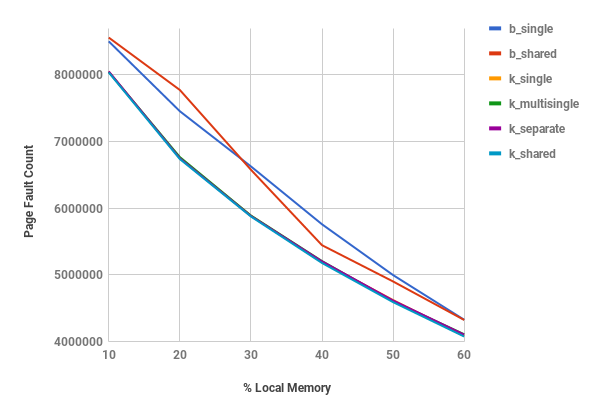
\includegraphics[width=\textwidth]{evaluation/compare_pf_redis.png}
		\caption{}
		\label{fig:compare_pf_redis}
	\end{subfigure}
	\begin{subfigure}[t]{\textwidth}
		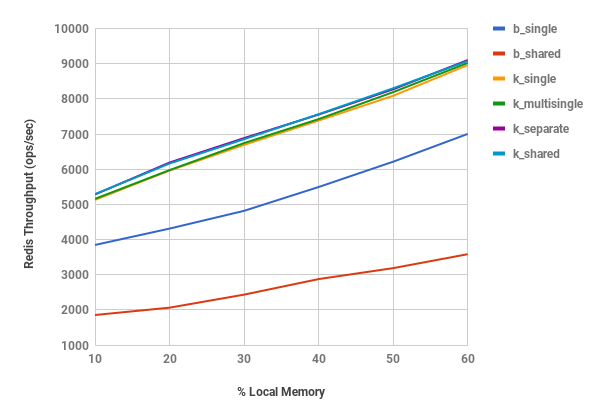
\includegraphics[width=\textwidth]{evaluation/compare_tp_redis.png}
		\caption{}
		\label{fig:compare_tp_redis}
	\end{subfigure}
	\caption{Redis performance comparison (Refer Table \ref{tab:graph_legends} for legends)}
	\label{fig:compare_redis}
\end{figure}

\begin{figure}[t]
	\centering
	
	\begin{subfigure}[t]{\textwidth}
		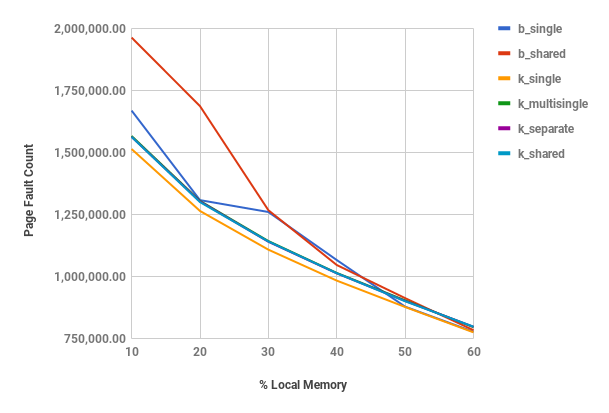
\includegraphics[width=\textwidth]{evaluation/compare_pf_memcached.png}
		\caption{}
		\label{fig:compare_pf_memcached}
	\end{subfigure}
	\begin{subfigure}[t]{\textwidth}
		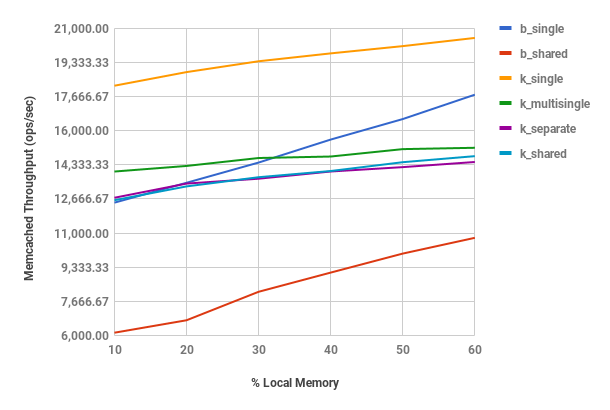
\includegraphics[width=\textwidth]{evaluation/compare_tp_memcached.png}
		\caption{}
		\label{fig:compare_tp_memcached}
	\end{subfigure}
	\caption{Memcached performance comparison (Refer Table \ref{tab:graph_legends} for legends)}
	\label{fig:compare_memcached}
\end{figure}
